\documentclass[dvisvgm,border=0pt]{standalone}
\usepackage[T1]{fontenc}
\usepackage{newtxtext,newtxmath}
\usepackage{tikz}
\usetikzlibrary{arrows.meta,decorations.pathmorphing}

\definecolor{Navy}{HTML}{08154F}
\definecolor{Ink}{HTML}{2B5098}
\definecolor{Blue}{HTML}{315EDB}
\definecolor{BlueTint}{HTML}{DCEBFC}
\definecolor{Sage}{HTML}{568638}
\definecolor{SageTint}{HTML}{E7F2E1}
\definecolor{Gold}{HTML}{F3B122}
\definecolor{Ice}{HTML}{F3FAFF}
\definecolor{Rule}{HTML}{CAE1FA}
\definecolor{Muted}{HTML}{8B95AA}

\tikzset{
  state/.style={draw=Blue,fill=BlueTint,line width=3bp,rounded corners=10bp},
  operation/.style={draw=Sage,fill=SageTint,line width=3bp,rounded corners=10bp},
  wire/.style={draw=Blue,line width=3bp,line cap=round,line join=round},
  blue arrow/.style={wire,-{Stealth[length=13bp,width=12bp]}},
  gold arrow/.style={draw=Gold,line width=6bp,line cap=round,-{Stealth[length=19bp,width=20bp]}},
  time arrow/.style={draw=Muted,line width=3bp,-{Stealth[length=17bp,width=15bp]}},
}

\newcommand{\figbackground}[2]{
  \path[use as bounding box] (0,0) rectangle (#1,#2);
  \fill[Ice!45] (0,0) rectangle (#1,#2);
}

\newcommand{\figtext}[5][Navy]{
  \node[text=#1,font=\fontsize{#4}{#4}\selectfont,inner sep=0bp,align=center]
    at (#2,#3) {#5};
}

\newcommand{\figmath}[5][Navy]{
  \figtext[#1]{#2}{#3}{#4}{$\displaystyle #5$}
}

\newcommand{\panelheading}[3]{
  \fill[BlueTint] (#1,190) circle (35bp);
  \node[text=Navy,font=\fontsize{40}{42}\selectfont\bfseries,inner sep=0bp]
    at (#1,190) {#2};
  \node[text=Navy,anchor=west,font=\fontsize{40}{42}\selectfont\bfseries,inner sep=0bp]
    at ({#1+62},190) {#3};
}

\newcommand{\panelrules}{
  \draw[Rule,line width=2bp] (535,162) -- (535,733);
  \draw[Rule,line width=2bp] (1090,162) -- (1090,733);
}

\newcommand{\statebox}[4]{
  \fill[Blue,opacity=.08,rounded corners=10bp]
    ({#1+4},{#2+6}) rectangle ({#3+4},{#4+6});
  \draw[state] (#1,#2) rectangle (#3,#4);
}

\newcommand{\operationbox}[4]{
  \fill[Sage,opacity=.08,rounded corners=10bp]
    ({#1+4},{#2+6}) rectangle ({#3+4},{#4+6});
  \draw[operation] (#1,#2) rectangle (#3,#4);
}

\newcommand{\processstrip}[4]{
  \fill[BlueTint!70,rounded corners=20bp] (50,762) rectangle (1622,858);
  \foreach \x/\word in {132/#1,522/#2,912/#3,1302/#4} {
    \fill[BlueTint,rounded corners=15bp] (\x,781) rectangle ({\x+306},837);
    \node[text=Navy,font=\fontsize{30}{34}\selectfont\bfseries,inner sep=0bp]
      at ({\x+153},809) {\word};
  }
  \foreach \x in {465,855,1245} {
    \draw[gold arrow] (\x,809) -- ({\x+31},809);
  }
}

\usepgflibrary{fpu}

% Introductory example and analytic profiles: arXiv:2603.06363v2, Appendix A.
% Growth classes: Sections III--IV. The global parity remains conserved.
\newcommand{\storyheading}[3]{
  \fill[BlueTint] (90,#1) circle (35bp);
  \node[text=Navy,font=\fontsize{40}{42}\selectfont\bfseries,inner sep=0bp]
    at (90,#1) {#2};
  \node[text=Navy,anchor=west,font=\fontsize{40}{42}\selectfont\bfseries,inner sep=0bp]
    at (152,#1) {#3};
}
\newcommand{\xspin}[3]{
  \fill[Blue,opacity=.08] (#1+3,#2+5) circle (22bp);
  \draw[draw=Blue,fill=BlueTint,line width=3bp] (#1,#2) circle (22bp);
  \draw[draw=Blue,line width=3bp,-{Stealth[length=10bp,width=9bp]}]
    ({#1-12*#3},#2) -- ({#1+12*#3},#2);
}

\begin{document}
\begin{tikzpicture}[x=1bp,y=-1bp]
  \figbackground{1672}{2140}
  \figtext[Ink]{836}{85}{38}{Strong-to-weak spontaneous symmetry breaking}

  % 1. A concrete local-versus-global explanation, using the ZZ example.
  \storyheading{190}{01}{What is SWSSB?}
  \figtext[Ink]{836}{252}{32}{A mixed quantum state can carry order that ordinary correlations miss}
  \figtext{275}{312}{35}{\textbf{Strong symmetry locally}}
  \figtext{1225}{312}{35}{\textbf{Weak symmetry locally}}
  \figtext[Muted]{1225}{340}{23}{Late-time mixed state}
  \figmath{275}{373}{33}{\lvert\psi_0\rangle=\lvert{+x}\rangle^{\otimes L}}
  \figtext[Muted]{275}{404}{23}{Schematic chain}

  % Highlight a two-site block A. Its parity is sharp initially.
  \fill[BlueTint!65,rounded corners=12bp] (61,412) rectangle (198,496);
  \draw[Rule,line width=4bp] (88,454) -- (513,454);
  \foreach \x in {88,173,258,343,428,513} {\xspin{\x}{454}{1}}
  \figtext[Ink]{129}{521}{28}{Region $A$}
  \figmath{275}{576}{35}{X_A\rho_A=\rho_A}
  \figtext[Ink]{275}{630}{30}{Its local parity is fixed}

  % Pair flips preserve the global X parity but mix local charge sectors.
  \operationbox{610}{366}{861}{425}
  \figtext{736}{395}{31}{Pair dephasing}
  \draw[gold arrow] (615,466) -- (853,466);
  \figmath{736}{522}{30}{L_j=\sqrt{\gamma}\,Z_jZ_{j+1}}
  \figtext[Ink]{736}{580}{28}{Open-system dynamics}

  % Representative X-basis configurations from the even-parity ensemble.
  % Three rows are examples; the dots indicate the remaining configurations.
  \fill[SageTint,rounded corners=12bp] (913,379) rectangle (1060,614);
  \figtext[Ink]{1450}{352}{25}{Local}
  \figtext[Ink]{1570}{352}{25}{Global}
  \figmath{1450}{379}{28}{X_A}
  \figmath{1570}{379}{28}{X}
  \foreach \y in {426,509,592} {
    \draw[Rule,line width=4bp] (938,\y) -- (1338,\y);
  }
  \foreach \x in {938,1018,1098,1178,1258,1338} {\xspin{\x}{426}{1}}
  \foreach \x/\s in {938/1,1018/-1,1098/1,1178/-1,1258/1,1338/1} {
    \xspin{\x}{509}{\s}
  }
  \foreach \x/\s in {938/-1,1018/1,1098/-1,1178/1,1258/1,1338/1} {
    \xspin{\x}{592}{\s}
  }
  \figmath[Sage]{1450}{426}{35}{+}
  \figmath[Sage]{1450}{509}{35}{-}
  \figmath[Sage]{1450}{592}{35}{-}
  \foreach \y in {426,509,592} {\figmath{1570}{\y}{35}{+}}
  \figtext[Ink]{1138}{636}{27}{Examples from the ensemble $\cdots$}
  \figmath{1225}{686}{35}{X_A\rho_A X_A=\rho_A}
  \figtext[Ink]{1225}{731}{29}{The local ensemble stays invariant}
  \figtext[Muted]{275}{684}{25}{Arrows: local $X_j=\pm1$ eigenstates}
  \figmath[Ink]{275}{732}{26}{\textstyle X_A=\prod_{j\in A}X_j,\quad X=\prod_jX_j}

  \fill[BlueTint!65,rounded corners=15bp] (50,765) rectangle (1622,820);
  \figtext{836}{793}{31}{Local parity fluctuates; global parity stays conserved}

  % 2. Large waterfall plot, following the user's reference composition.
  \draw[Rule,line width=2bp] (50,861) -- (1622,861);
  \storyheading{926}{02}{Watch the nonlinear order spread}
  \figtext[Ink]{836}{984}{30}{Each ridge is a later snapshot of the same chain}

  % Affine 3D projection: signed site displacement r, increasing time k,
  % and R2 height. Draw back-to-front so every ridge remains visible.
  % Exact open-chain ZZ-dephasing profiles: R2=[tanh(2 gamma t)]^|r|.
  \begin{scope}
  \pgfkeys{/pgf/fpu=true,/pgf/fpu/output format=fixed}
  \foreach \k in {6,5,4,3,2,1,0} {
    \pgfmathsetmacro{\s}{0.30+0.15*\k}
    \pgfmathsetmacro{\q}{(exp(4*\s)-1)/(exp(4*\s)+1)}
    \fill[BlueTint!80!white]
      ({580-480+27*\k},{1510-80-30*\k})
      -- plot[domain=-40:40,samples=161,variable=\r]
        ({580+12*\r+27*\k},{1510+2*\r-30*\k-300*pow(\q,abs(\r))})
      -- ({580+480+27*\k},{1510+80-30*\k}) -- cycle;
    \draw[Blue,line width=3bp,line cap=round,line join=round]
      plot[domain=-40:40,samples=161,variable=\r]
        ({580+12*\r+27*\k},{1510+2*\r-30*\k-300*pow(\q,abs(\r))});
    \draw[Rule,line width=1bp]
      ({580-480+27*\k},{1510-80-30*\k})
      -- ({580+480+27*\k},{1510+80-30*\k});
  }
  \end{scope}

  % Axes have quantitative ticks for these analytic profiles.
  \draw[time arrow] (100,1430) -- (1086,1594);
  \draw[time arrow] (580,1510) -- (780,1287);
  \draw[time arrow] (580,1510) -- (580,1185);
  \foreach \r in {-40,-20,0,20,40} {
    \draw[Muted,line width=2bp]
      ({580+12*\r},{1510+2*\r}) -- ({580+12*\r},{1518+2*\r});
    \figmath{580+12*\r}{1548+2*\r}{28}{\r}
  }
  \figmath{1125}{1629}{35}{r}
  \foreach \z in {0,0.5,1} {
    \draw[Muted,line width=2bp] (573,{1510-300*\z}) -- (587,{1510-300*\z});
    \figmath{543}{1510-300*\z}{27}{\z}
  }
  \figmath{566}{1152}{35}{R_2(r,t)}
  \foreach \k/\s in {0/0.3,2/0.6,4/0.9,6/1.2} {
    \draw[Muted,line width=2bp]
      ({580+27*\k-5},{1510-30*\k-4})
      -- ({580+27*\k+5},{1510-30*\k+4});
    \figmath{623+27*\k}{1523-30*\k}{25}{\s}
  }
  \figmath{820}{1287}{32}{\gamma t}
  \figtext[Ink]{304}{1556}{27}{Early: a narrow profile}

  % Explain the nonlinear diagnostic and absence of ordinary order.
  \figtext{1441}{1112}{33}{\textbf{Hidden long-range order}}
  \figtext[Ink]{1441}{1164}{28}{Broader ridges mean\\a longer correlation range}
  \figmath{1441}{1241}{29}{R_2(r,t)=e^{-|r|/\xi(t)}}
  \figmath{1441}{1304}{30}{\xi(t)\sim\tfrac12 e^{4\gamma t}}
  \figtext[Ink]{1441}{1374}{28}{Ordinary correlations\\stay absent in this example}
  \draw[time arrow] (1270,1450) -- (1605,1450);
  \draw[time arrow] (1270,1450) -- (1270,1409);
  \draw[Blue,line width=4bp] (1280,1448) -- (1591,1448);
  \figmath{1441}{1498}{31}{C_Z(r>0,t)=0}
  \figmath{1605}{1481}{27}{r}
  \figtext[Muted]{1441}{1556}{25}{No conventional $Z$-spin alignment}

  \figmath{836}{1680}{32}{
    R_2(r,t)=\frac{\operatorname{Tr}[\rho(t)Z_iZ_j\rho(t)Z_jZ_i]}
    {\operatorname{Tr}[\rho(t)^2]},\qquad r=i-j
  }
  \figtext[Ink]{836}{1745}{28}{Two copies of the density matrix reveal what a single-copy correlator misses}

  % 3. A compact comparison; most space explains SWSSB itself.
  \draw[Rule,line width=2bp] (50,1793) -- (1622,1793);
  \storyheading{1854}{03}{Our result: symmetry sets the pace}
  \figtext{450}{1916}{32}{\textbf{$\mathbb{Z}_2$: exponential, including gapless models}}
  \figmath[Sage]{450}{1971}{37}{\xi_{R_2}\sim e^{\lambda t},\qquad t_c\sim\ln L}
  \figtext{1250}{1916}{32}{\textbf{$U(1)$: algebraic}}
  \figmath[Blue]{1250}{1971}{32}{
    \xi_{R_2}\sim t,\ t_c\sim L\quad\text{(finite filling)}
  }
  \figmath[Gold!80!Navy]{1250}{2016}{30}{
    \xi_{R_2}\sim\sqrt{t},\ t_c\sim L^2\quad\text{(single particle / hole)}
  }
  \figtext[Muted]{836}{2053}{23}{Pair-dephasing example: Appendix A $\cdot$ Symmetry-dependent scaling: Sections III--IV}
  \figtext[Muted]{836}{2095}{26}{Finite chains: onset at $\xi_{R_2}\sim L$. Infinite chains: long-range order emerges only as $t\to\infty$.}
\end{tikzpicture}
\end{document}
